%%%%%%%%%%%%%%%%%%%%%%%%%%%%%%%%%%%%%%%%%
% Beamer Presentation
% LaTeX Template
% Version 1.0 (10/11/12)
%
% This template has been downloaded from:
% http://www.LaTeXTemplates.com
%
% License:
% CC BY-NC-SA 3.0 (http://creativecommons.org/licenses/by-nc-sa/3.0/)
%
%%%%%%%%%%%%%%%%%%%%%%%%%%%%%%%%%%%%%%%%%

\documentclass{beamer}

\mode<presentation> {

\usetheme{Madrid}
%\usecolortheme{beaver}

\setbeamertemplate{caption}[numbered]
}

\usepackage{graphicx} % Allows including images
\usepackage{booktabs} % Allows the use of \toprule, \midrule and \bottomrule in tables

% code blocks
\usepackage{minted} % yaml
\usepackage{listings}
\usepackage{xcolor}

\definecolor{codegreen}{rgb}{0,0.6,0}
\definecolor{codegray}{rgb}{0.5,0.5,0.5}
\definecolor{codepurple}{rgb}{0.58,0,0.82}
\definecolor{backcolour}{rgb}{0.95,0.95,0.92}

\lstdefinestyle{mystyle}{
    backgroundcolor=\color{backcolour},   
    commentstyle=\color{codegreen},
    keywordstyle=\color{magenta},
    numberstyle=\tiny\color{codegray},
    stringstyle=\color{codepurple},
    basicstyle=\ttfamily\footnotesize,
    breakatwhitespace=false,         
    breaklines=true,                 
    captionpos=b,                    
    keepspaces=true,                 
    numbers=left,                    
    numbersep=5pt,                  
    showspaces=false,                
    showstringspaces=false,
    showtabs=false,                  
    tabsize=2
}
\lstset{style=mystyle}
%%%%
\usepackage{nameref}

\makeatletter
\newcommand*{\currentname}{\@currentlabelname}
\makeatother

%----------------------------------------------------------------------------------------
%	TITLE PAGE
%----------------------------------------------------------------------------------------
%\title[Projeto Integrador 3]{Projeto Integrador 3}
%\author{Leonardo Benitez}
%\institute[IFSC]{Instituto Federal de Santa Catarina \\ \medskip\textit{lsBenitezPereira@gmail.com}}
\title[DIA Project]{DIA Project}
%Digital Innovation aceleration
\author{Leonardo Benitez}
\institute[Skaylink]{Skaylink \\
\medskip\textit{leonardo.benitez@skaylink.com}}
\date{\today} % Date, can be changed to a custom date

\begin{document}

\begin{frame}
\titlepage % Print the title page as the first slide
\end{frame}

\begin{frame}
\frametitle{Overview} % Table of contents slide, comment this block out to remove it
\tableofcontents % Throughout your presentation, if you choose to use \section{} and \subsection{} commands, these will automatically be printed on this slide as an overview of your presentation
\end{frame}



%%%%%%%%%%%%%%%%%%%%%%%%%%%%%%%%%%%%%%%%
\section{Introduction}
\begin{frame}
\centering \Huge {\secname}
\end{frame}

\begin{frame}
\frametitle{\secname}
\begin{itemize}
\item Joint innovation project between Skaylink and KWS.
\item Skaylink: consultoria e desenvolvimento de projetos.
\item KWS: produtor de sementes (4º maior do mundo)
\end{itemize}

\begin{center}
\begin{columns}[c]
\column{.5\textwidth} % Left column and width
\begin{figure}

\includegraphics[width=0.5\linewidth]{Imagens/skaylink.png}
\end{figure}

\column{.5\textwidth} % Right column and width
\begin{figure}

\includegraphics[width=0.3\linewidth]{Imagens/kws.png}
\end{figure}
\end{columns}\end{center}
\end{frame}

\subsection{Problem definition}
\begin{frame}
\frametitle{\secname\ - \subsecname}
\begin{columns}[c]
\column{.5\textwidth} % Left column and width
\begin{figure}
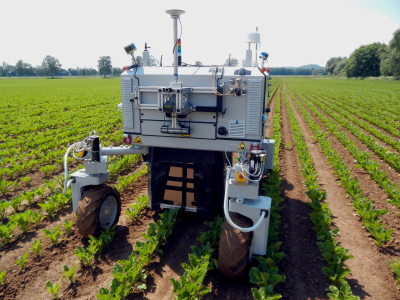
\includegraphics[width=1\linewidth]{Imagens/unibonn.png}
\end{figure}
\center{Unibonn research robot}

\column{.5\textwidth} % Right column and width
\begin{figure}
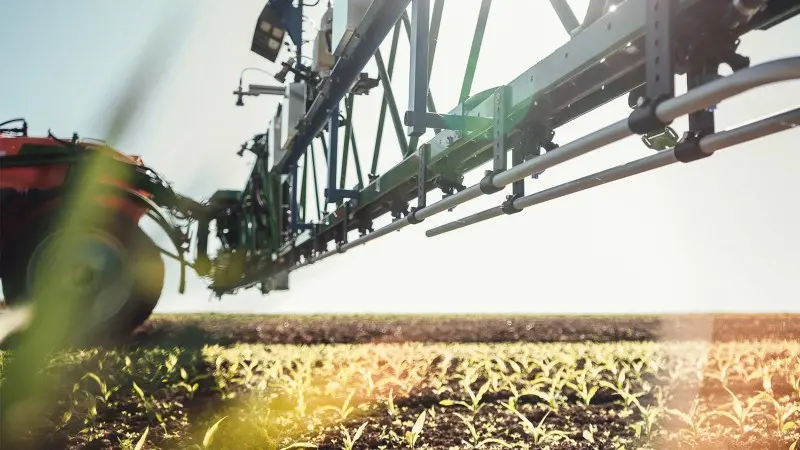
\includegraphics[width=1\linewidth]{Imagens/bosh.png}
\end{figure}
\center{Bosh smart spraying}
\end{columns}
\end{frame}

\begin{frame}
\frametitle{\secname\ - \subsecname}
\begin{itemize}
\item Explore new technologies.
\item Optimize operations, less human labour, increase yield.
\item There were 2 workshops with KWS where we had our initial conversation about the project, KWS's plans, initial brainstorming, etc.
%modelos de negócios alternativos, complementar àvenda de sementes; eles querem vender isso para os fazendeiros, otimizado para as sementes deles

%estão entrando no mercado de verduras e legumes

%a beterraba é difícil de fazer modificações genéticas


\end{itemize}
\begin{figure}
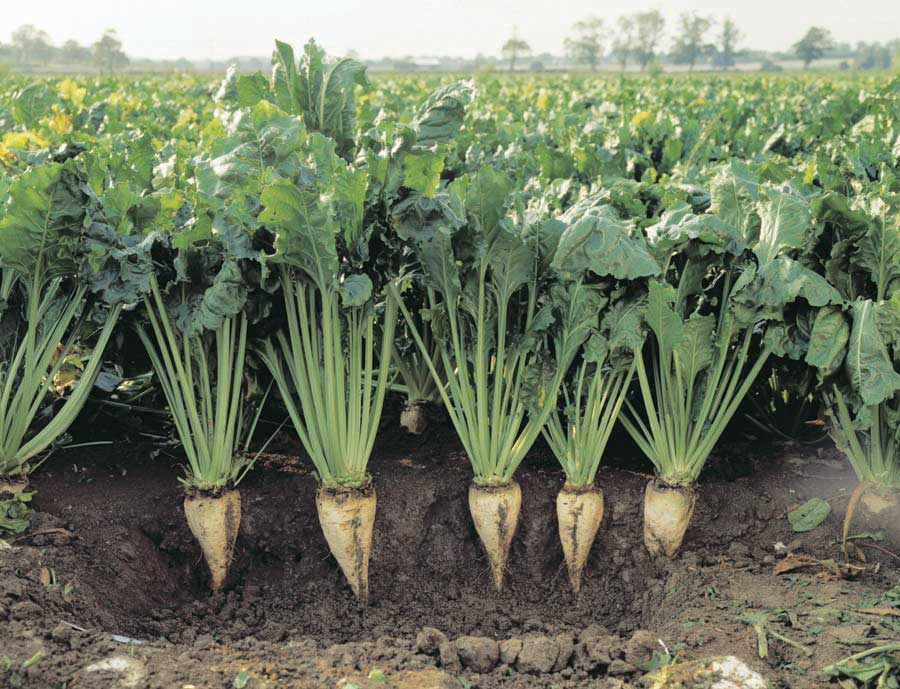
\includegraphics[width=0.4\linewidth]{Imagens/sugarbeet.png}
\end{figure}
\end{frame}




\subsection{Related technologies}
\begin{frame}
\frametitle{\secname\ - \subsecname}
\begin{itemize}
\item \textbf{Embedded Systems}
\begin{itemize}
    \item Dedicated processing system within a larger mechanical or electrical system
    \item ABS controller, smart frige processor, aviation autopilot, ... 
\end{itemize}
\item \textbf{Internet of Things}
\begin{itemize}
    \item Common physical devices connected to internet
    \item Building automation, connected transportation systems, ...
\end{itemize}
\item \textbf{Edge Computing}
\begin{itemize}
    \item Computation and storage near the sources
    \item Distribute the processing power as much as possible
\end{itemize}
\item \textbf{Computer vision}
\begin{itemize}
    \item Extract useful information from image/video
    \item Identify things, track/follow, ...
\end{itemize}
\item \textbf{Smart Farming}
\begin{itemize}
    \item A bunch of cool technologies applied to agriculture
    \item Precision agriculture, crop monitoring, ...
\end{itemize}
\end{itemize}
\end{frame}

\begin{frame}
\frametitle{\secname}
\begin{figure}
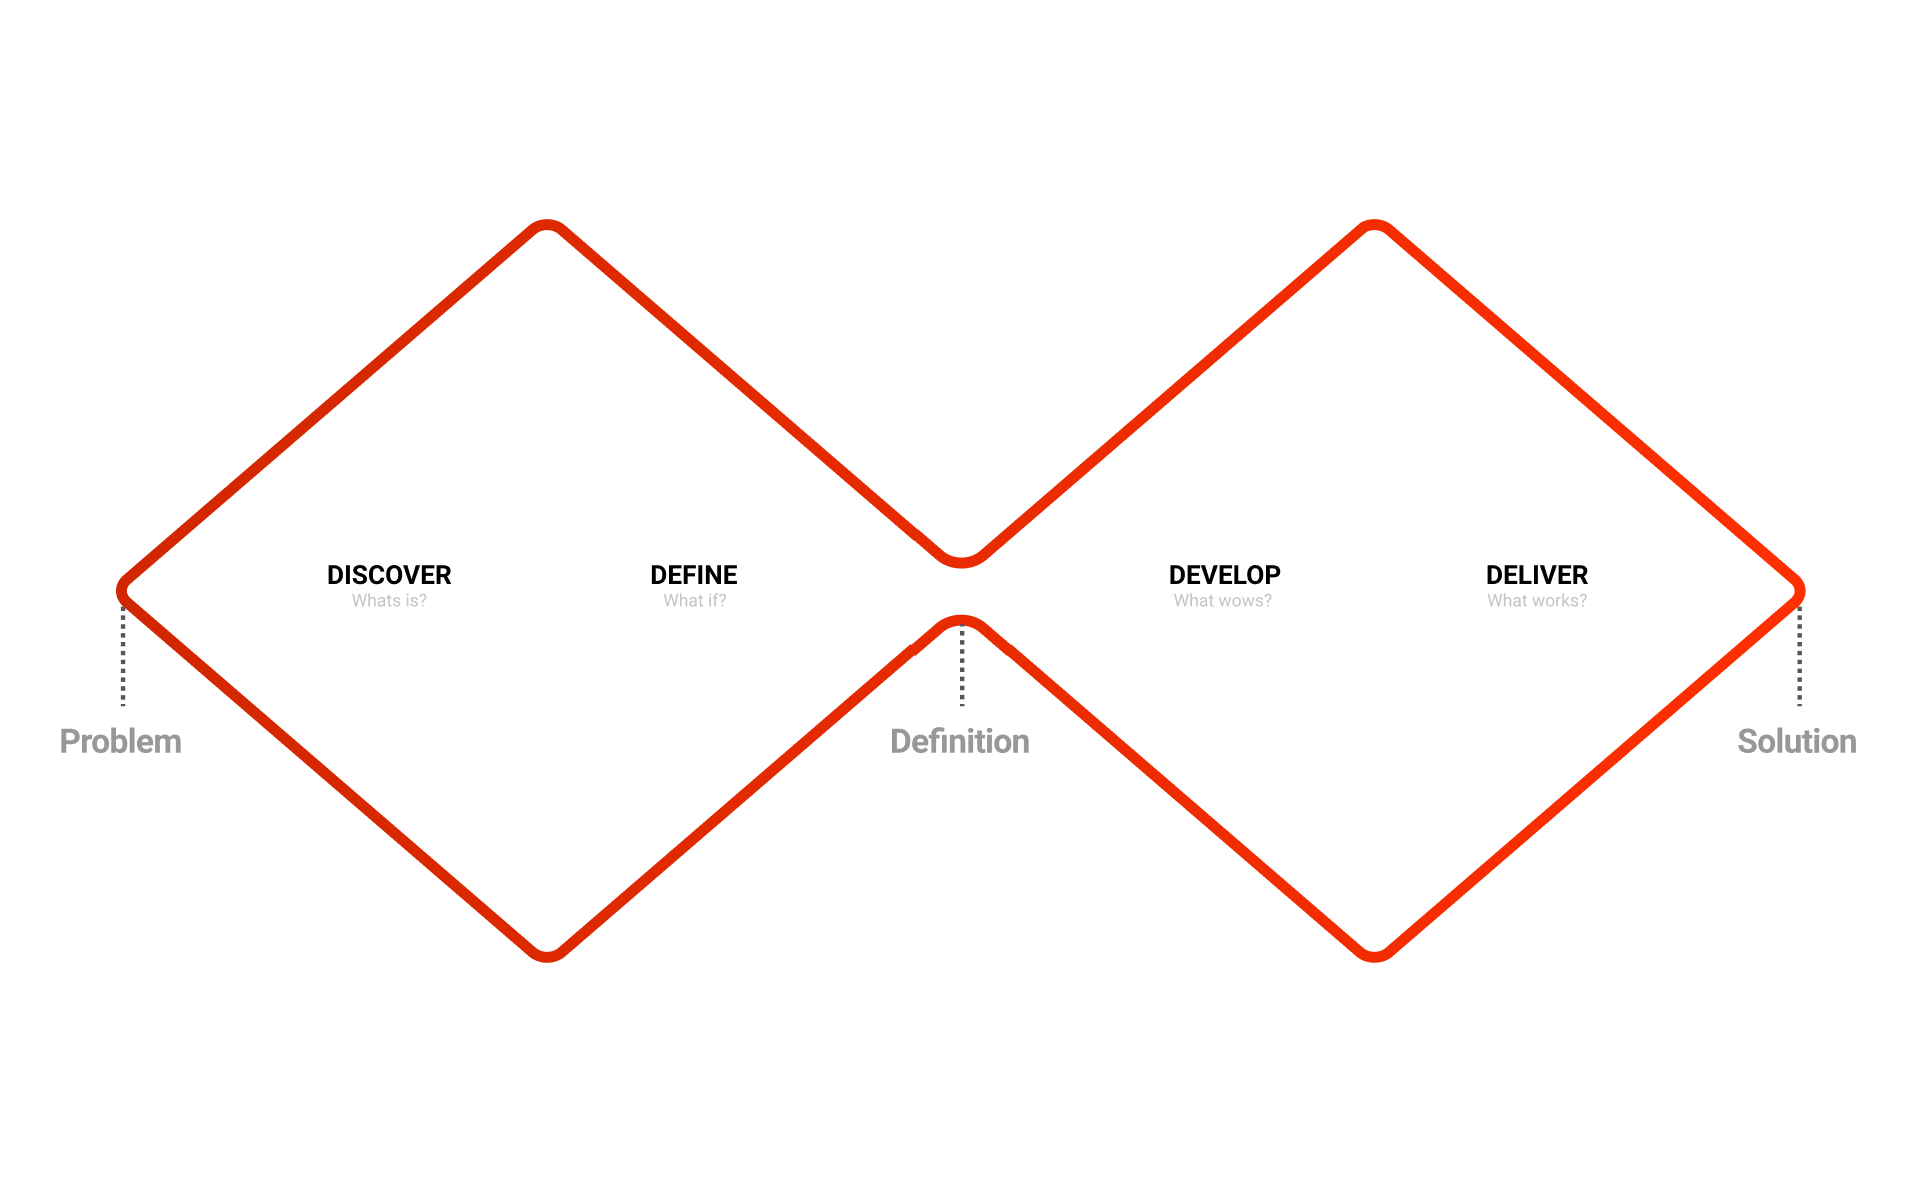
\includegraphics[width=0.9\linewidth]{Imagens/V1.png}
\end{figure}
\end{frame}


\begin{frame}
\frametitle{\secname}
\begin{figure}
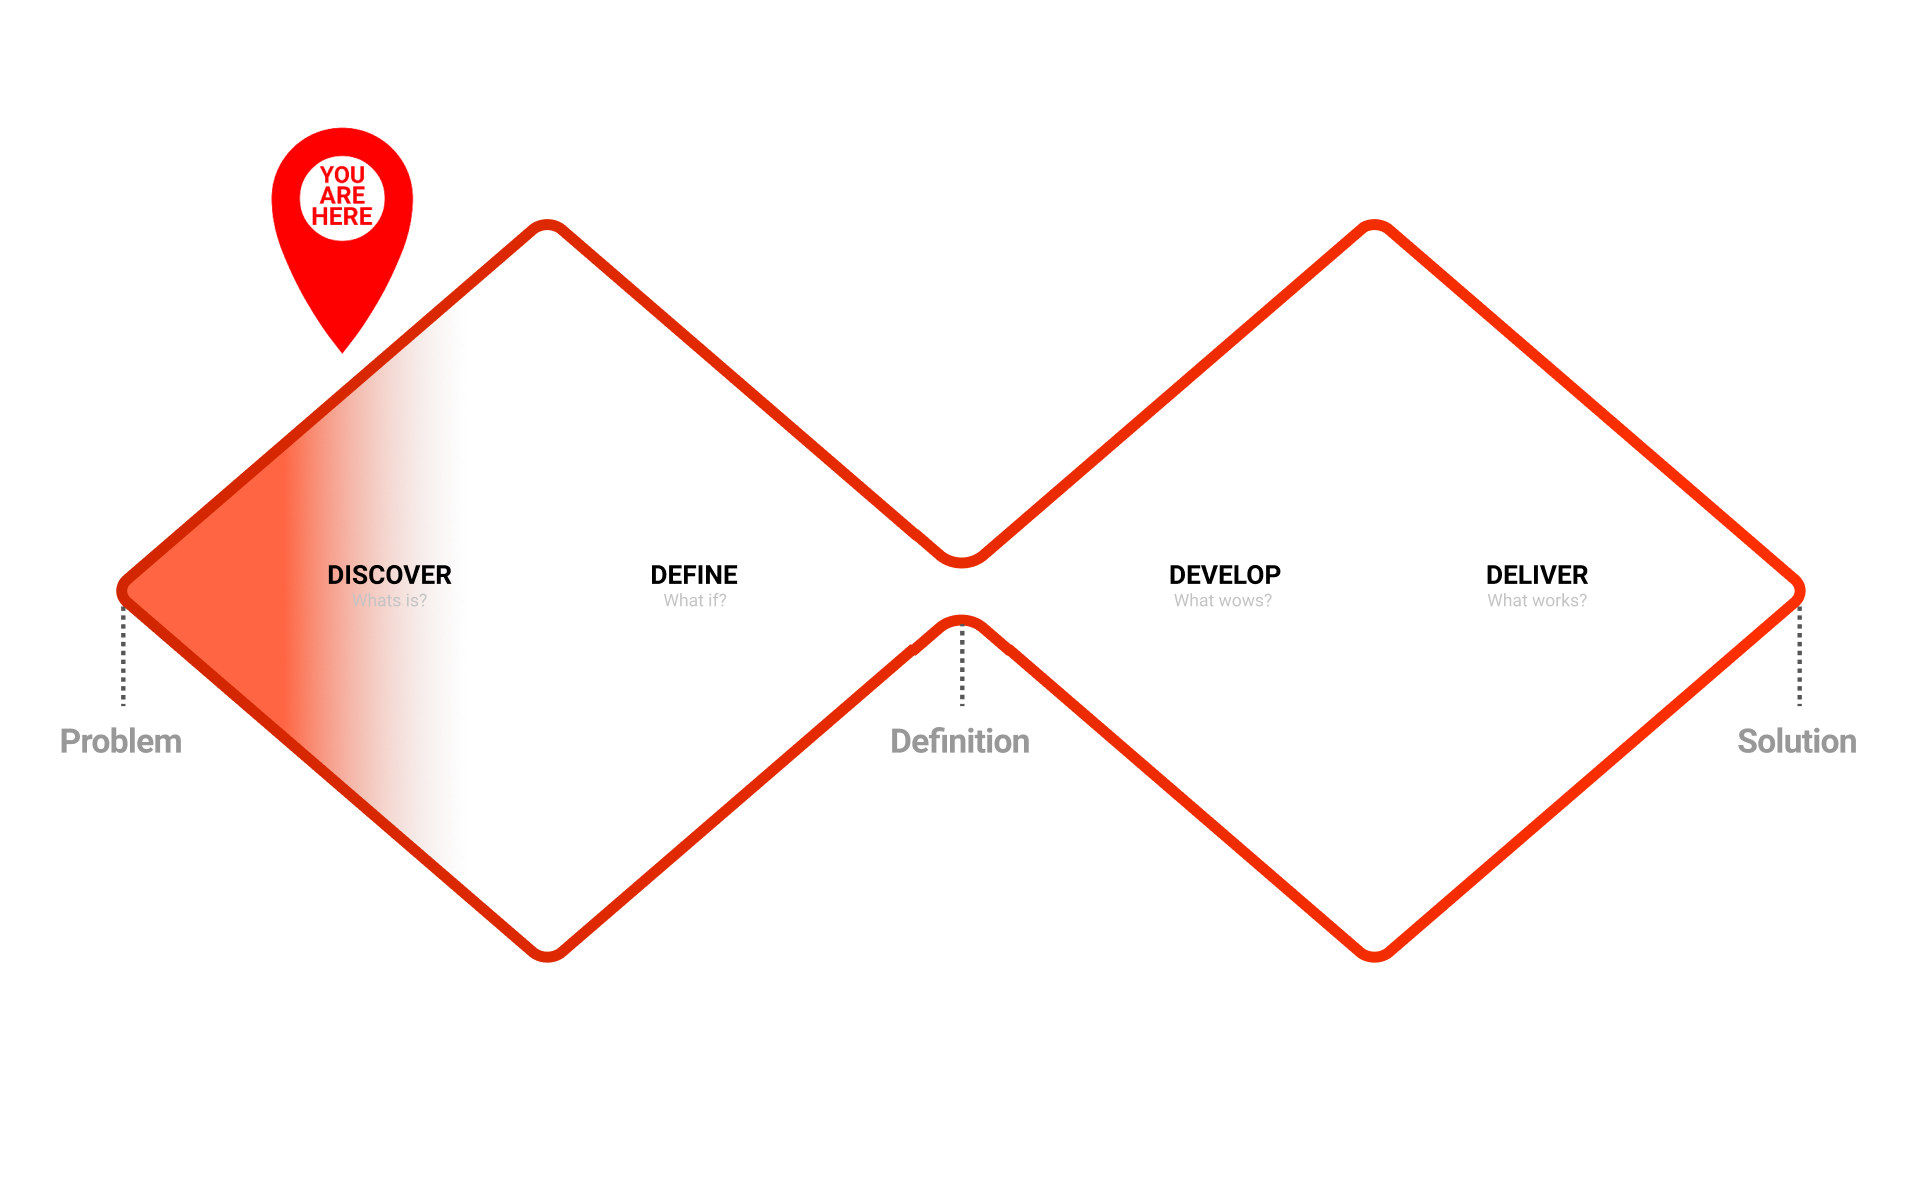
\includegraphics[width=0.9\linewidth]{Imagens/V1 A.jpg}
\end{figure}
\end{frame}



\subsection{Project definition}
\begin{frame}
\frametitle{\secname\ - \subsecname}
\begin{itemize}
\item Weed identification in plantation fields.
\item Top-notch object detection model (they already made a past project with another company).
\item Top-notch cloud architecture.
\item Proof of concept about the edge device.
\item Out of scope: method to remove/kill the weeds.
\item Out of scope: identify the type of the weed and growth stage (this would help with the pesticide amount).
\end{itemize}



\end{frame}




%%%%%%%%%%%%%%%%%%%%%%%%%%%%%%%%%%%%%%

\subsection{Requirements}
\begin{frame}
\frametitle{\secname\ - \subsecname}
\begin{itemize}
\item ML - Data collection and labeling.
\item ML - Model training and evaluation.
\item ML - Model deployment, both on cloud and edge.
\item IoT - take picture, include GPS information, upload to cloud.
\item IoT - if it is without internet, save image locally and retry later.
\end{itemize}
\end{frame}


\begin{frame}
\frametitle{\secname\ - \subsecname}
%Gestão dos dispositivos
\begin{itemize}
\item Remote update firmware
\item Secure connection with the cloud
\item Runtime log centralization
\item Support for diffenrent architectures: Raspberry pi (arm32) and jetson nano (arm64)
\item Add and shutdown devices easely
\item Cloud Infrastructure provisioning as code
\item Automated pipeline for software build, test and deploy
\end{itemize}
\textit{We can chose a service from azure/AWS/etc or build our own}
\end{frame}


\begin{frame}
\frametitle{\secname\ - \subsecname}
IoT Services Platform: provides abstraction across the multitude of diverse devices and data sources in addition to allowing for the management and control of a range of systems and processes (Rayes, 2019)

\begin{figure}
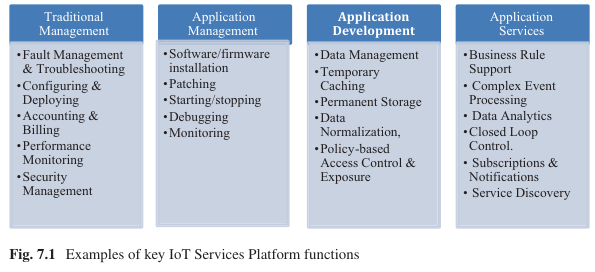
\includegraphics[width=0.9\linewidth]{Imagens/iot-service-platform.png}
\end{figure}

Comercial IoT  platforms: AWS greengrass, Azure IoT Hub, ...

\end{frame}



\begin{frame}
\frametitle{\secname}
\begin{figure}
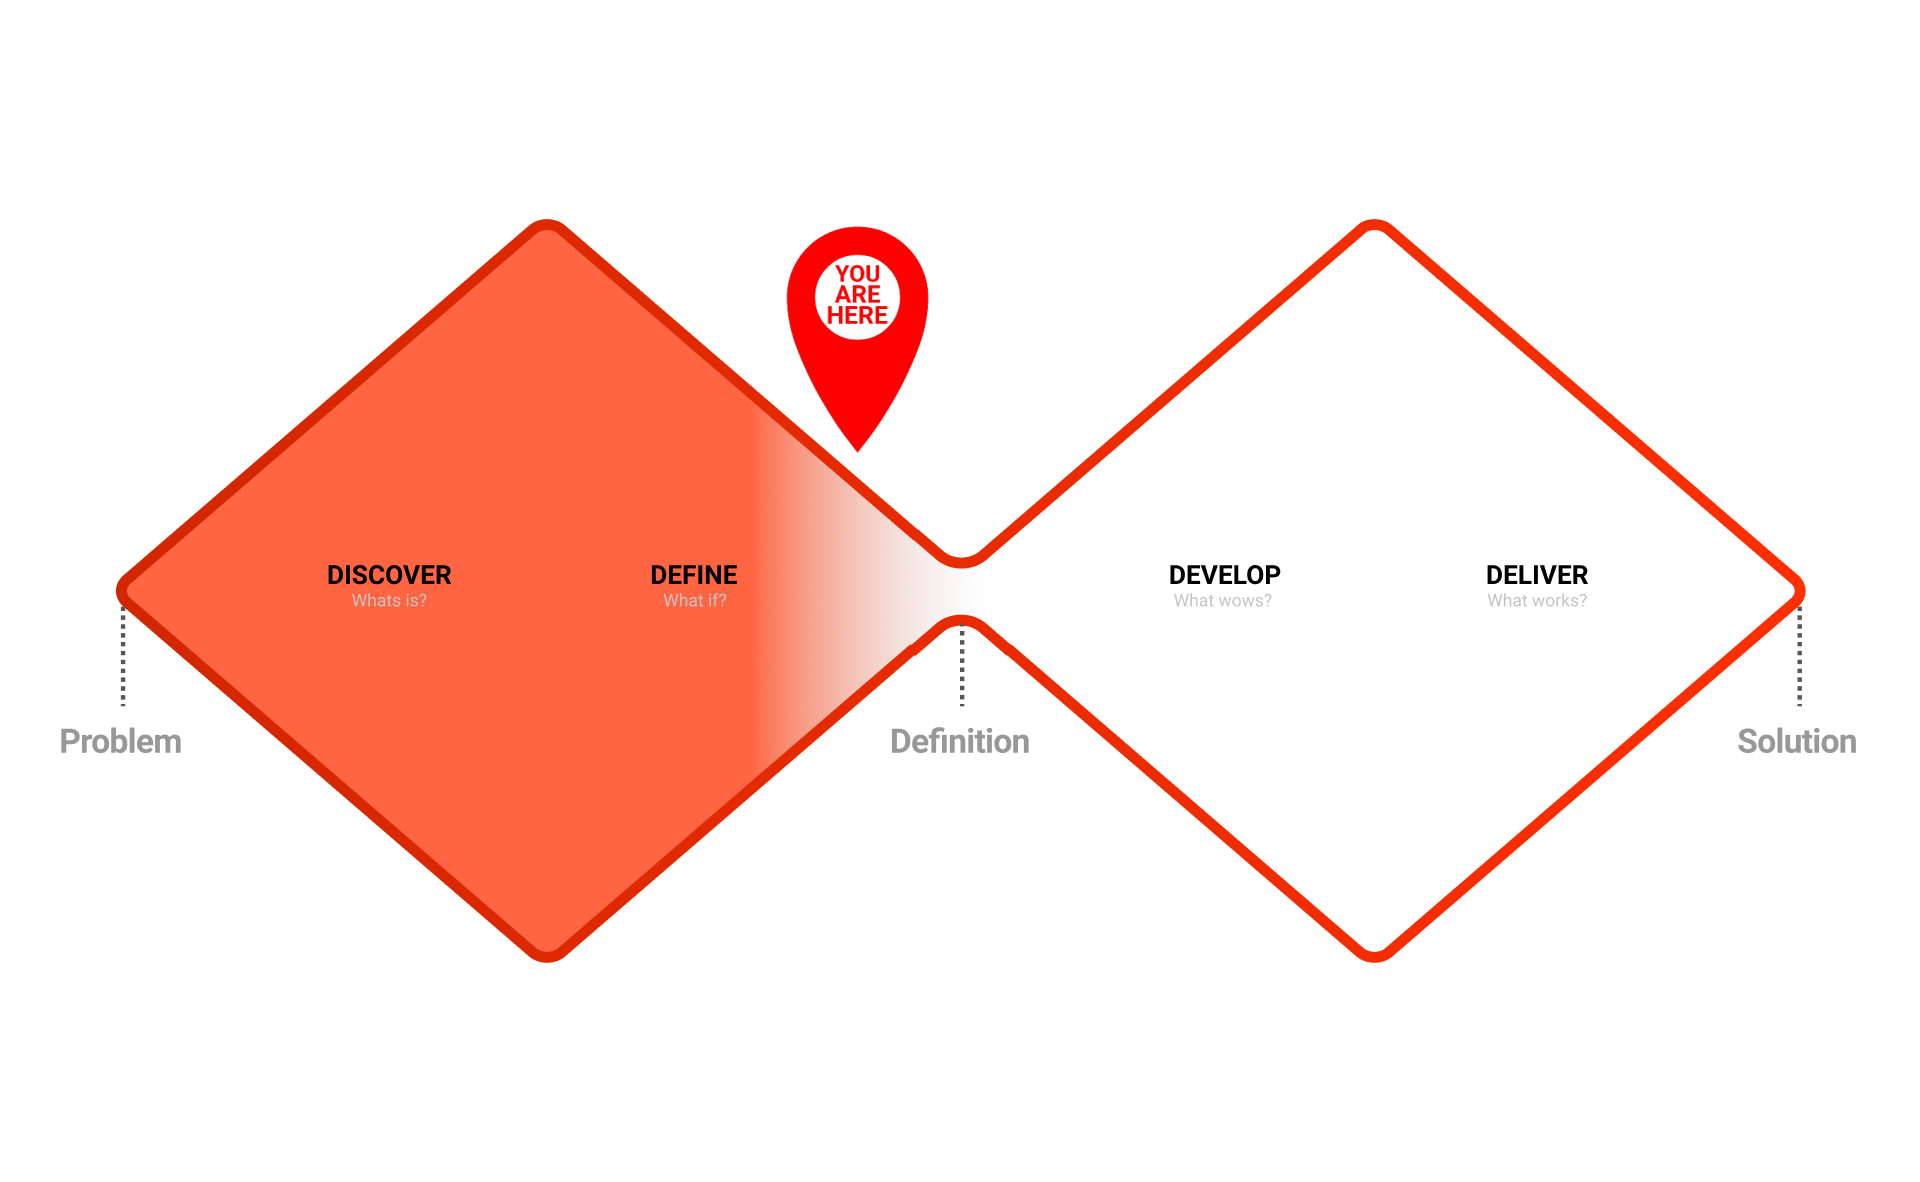
\includegraphics[width=0.9\linewidth]{Imagens/V1 B.jpg}
\end{figure}
\end{frame}


%%%%%%%%%%%%%%%%
\section{Implementation possibilities}
\begin{frame}
\centering \Huge {\currentname}
\end{frame}


\subsection{Architecture related}
\begin{frame}
\frametitle{\secname\ - \subsecname}
\begin{itemize}
\item \textbf{IoT platform}
\begin{itemize}
    \item Azure IoT hub
    \item AWS green grass
\end{itemize}
\item \textbf{Architecture}
\begin{itemize}
    \item Device access an inference API, and upload the results?
    \item Device access an inference + upload API?
    \item Device upload the raw images to blob storage, and inference is triggered on cloud?
\end{itemize}
\item \textbf{CI, CD and IaaS tooling}
\begin{itemize}
    \item Terraform, ARM templates, cloudformation...
    \item Azure pipelines, github actions...
\end{itemize}
\end{itemize}
\end{frame}

\subsection{Data related}
\begin{frame}
\frametitle{\secname\ - \subsecname}
\begin{itemize}
\item \textbf{Data collection}
\begin{itemize}
    \item KWS is providing images from their crop (Germany, Chile and US)
    \item There are public datasets, like the UniBonn dataset (Chebrolu Et al., 2017), but the images are usually very different from our + we may have problems with license
\end{itemize}
\item \textbf{Labeling stategy}
\begin{itemize}
    \item We actually only want to detect weed, should we label sugarbeets and weeds? or just weeds, or just sugarbeet?
    \item Should we label the whole contour or just the center?
    \item There are different types of weeds... should we label them all?
    \item Leaving some weeds undetected, or detect all the weeds and possibly kill a few sugarbets?
\end{itemize}
\item \textbf{Labeling tool}
\begin{itemize}
    \item Opensource web-based (Snorkel AI, Label studio), upload to website and label there
    \item Opensource offline (labelImg, VIA), install software and label locally
    \item Proprietary SaaS (Azure labeling service), extra features like automatic labeling
\end{itemize}
\end{itemize}
\end{frame}



\subsection{ML related}
\begin{frame}
\frametitle{\secname\ - \subsecname}
\begin{itemize}
\item \textbf{CV task type}
\begin{itemize}
    \item Image classification (background removal by color + ML classifier)
    \item Object detection (bounding boxes around each plant)
    \item Instance segmentation (shapes)
\end{itemize}
\item \textbf{Base model}
\begin{itemize}
    \item Detectron2, "barebore" pytorch
    \item Azure Custom Vision, still a code-first approach
    \item Azure AutoML, fully automated training
\end{itemize}
\item \textbf{Inference method}
\begin{itemize}
    \item On stream
    \item As a module
\end{itemize}
\end{itemize}
\end{frame}


\begin{frame}
\frametitle{\secname}
\begin{figure}
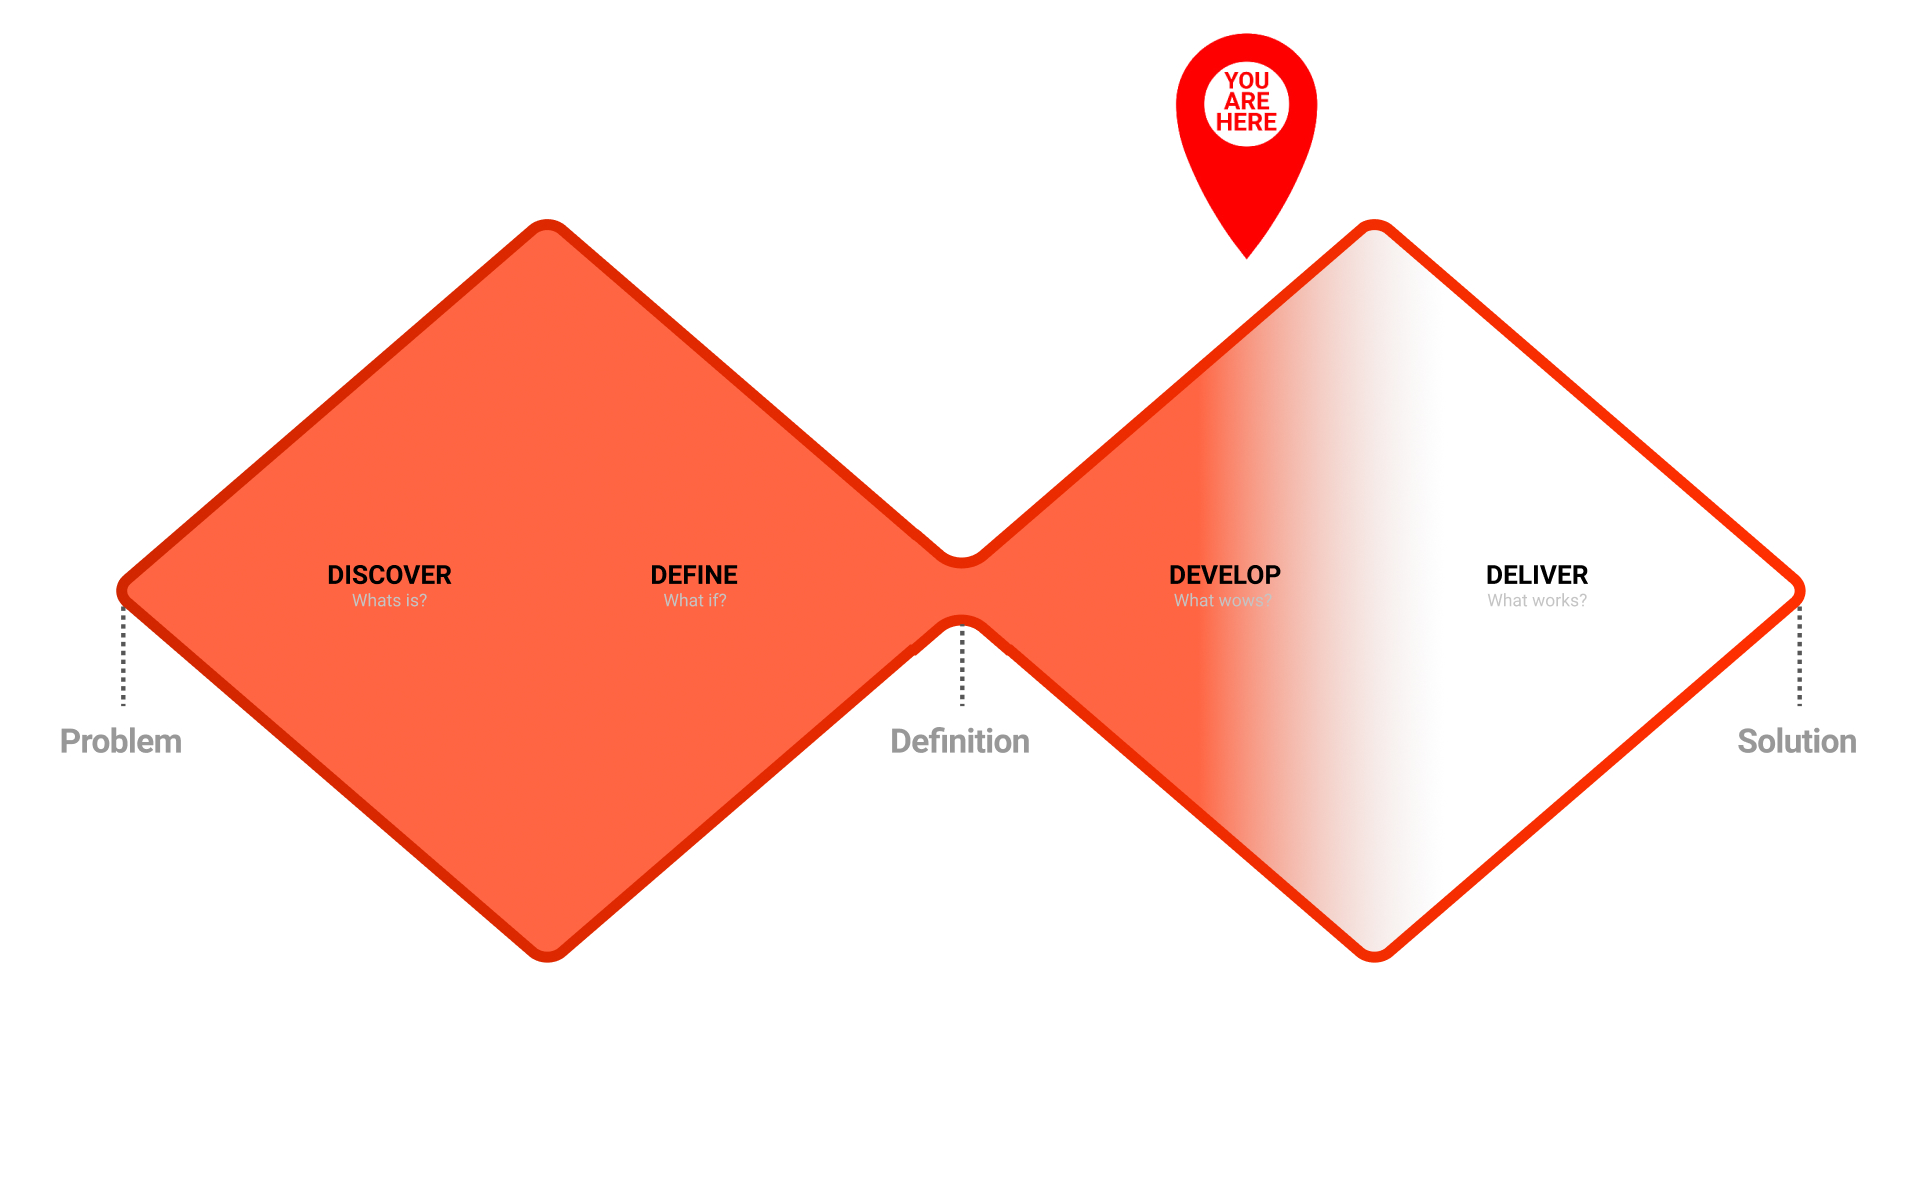
\includegraphics[width=0.9\linewidth]{Imagens/V1 C.jpg}
\end{figure}
\end{frame}

%%%%%%%%%%%%%%%%%%%%%%%%%%%
\section{Implemented solution}
\begin{frame}
\centering \Huge {\currentname}
\end{frame}

\begin{frame}
\frametitle{\secname}
\begin{itemize}
\item \textbf{IoT platform}: Azure IoT hub
\item \textbf{Architecture}: edge inference or cloud inference
\item \textbf{Tooling}: terraform + azure pipelines
\item \textbf{Data collection}: trained 100\% with our data, tested with Bonn dataset
\item \textbf{Labeling stategy}: 2 types of weed + sugarbeets, only when completely visible; 320 labeled images
\item \textbf{Labeling tool}: azure labeling service
\item \textbf{CV task type}: detection (bounding boxes)
\item \textbf{Base model}: azure AutoML
\item \textbf{Inference method}: as a module 
\item \textbf{Metric}: custom "beets kill vs weeds kill" 
\end{itemize}
\end{frame}

\begin{frame}
\frametitle{\currentname}
\begin{figure}
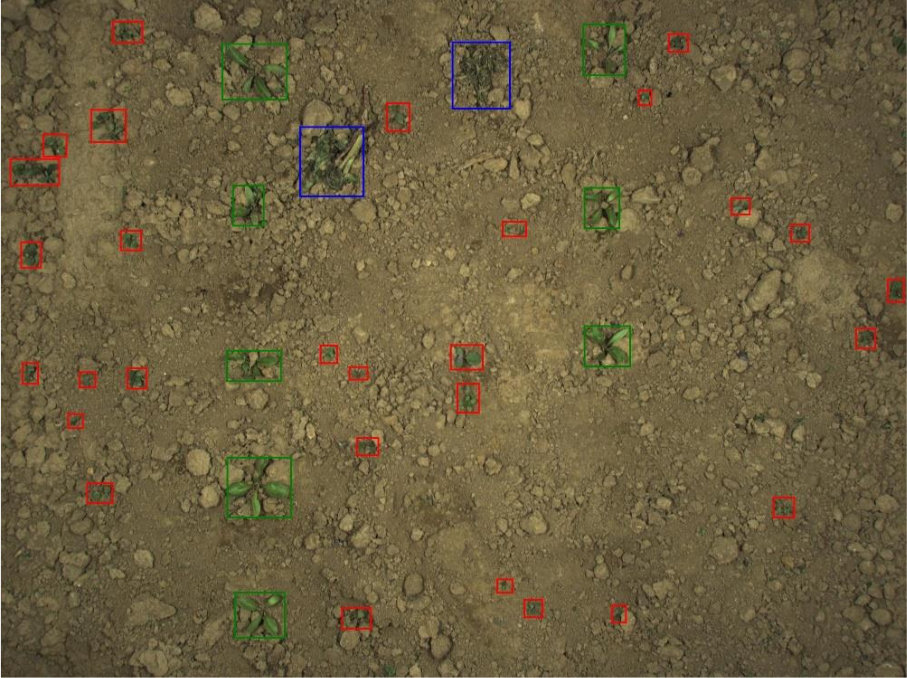
\includegraphics[width=0.9\linewidth]{Imagens/prediction.png}
\end{figure}
\end{frame}

\begin{frame}
\frametitle{\currentname}
\begin{figure}
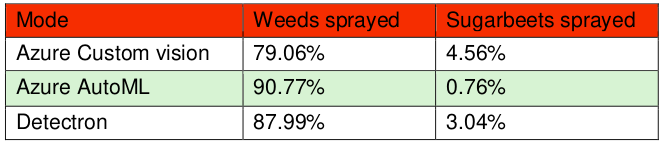
\includegraphics[width=0.9\linewidth]{Imagens/results_table.png}
\end{figure}

\begin{figure}
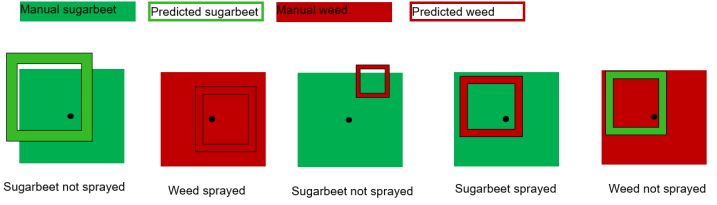
\includegraphics[width=0.9\linewidth]{Imagens/metric_explanation.png}
\end{figure}

\end{frame}

\begin{frame}
\frametitle{\currentname}
Same functionalities for both raspberry and jetson nano
\begin{figure}
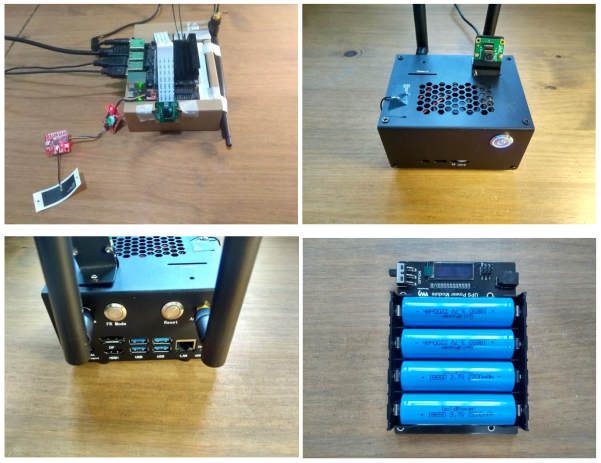
\includegraphics[width=0.7\linewidth]{Imagens/jetson.png}
\end{figure}
\end{frame}

\begin{frame}
\frametitle{\currentname}
\begin{figure}
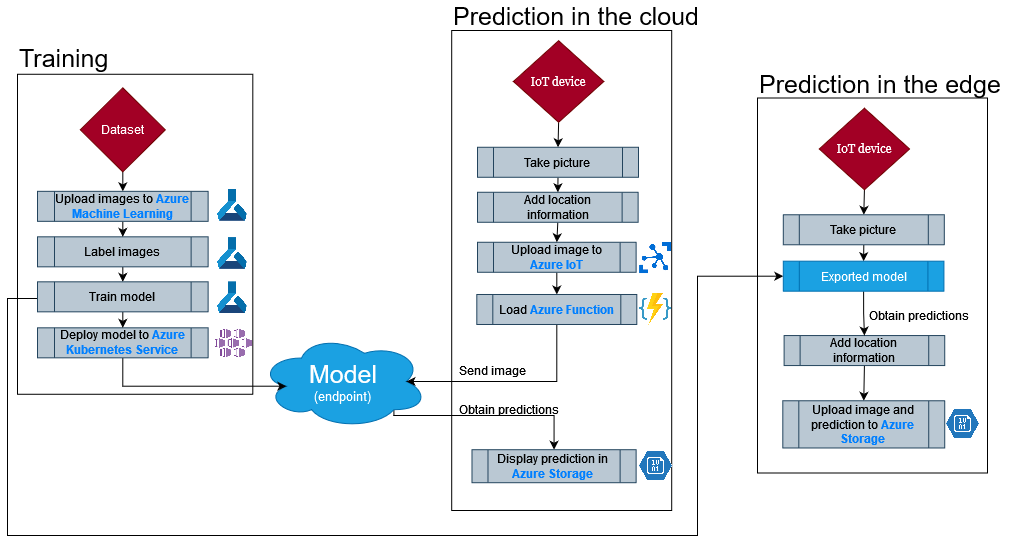
\includegraphics[width=1\linewidth]{Imagens/workflow.png}
\end{figure}
\end{frame}

\begin{frame}
\frametitle{\secname}
\begin{figure}
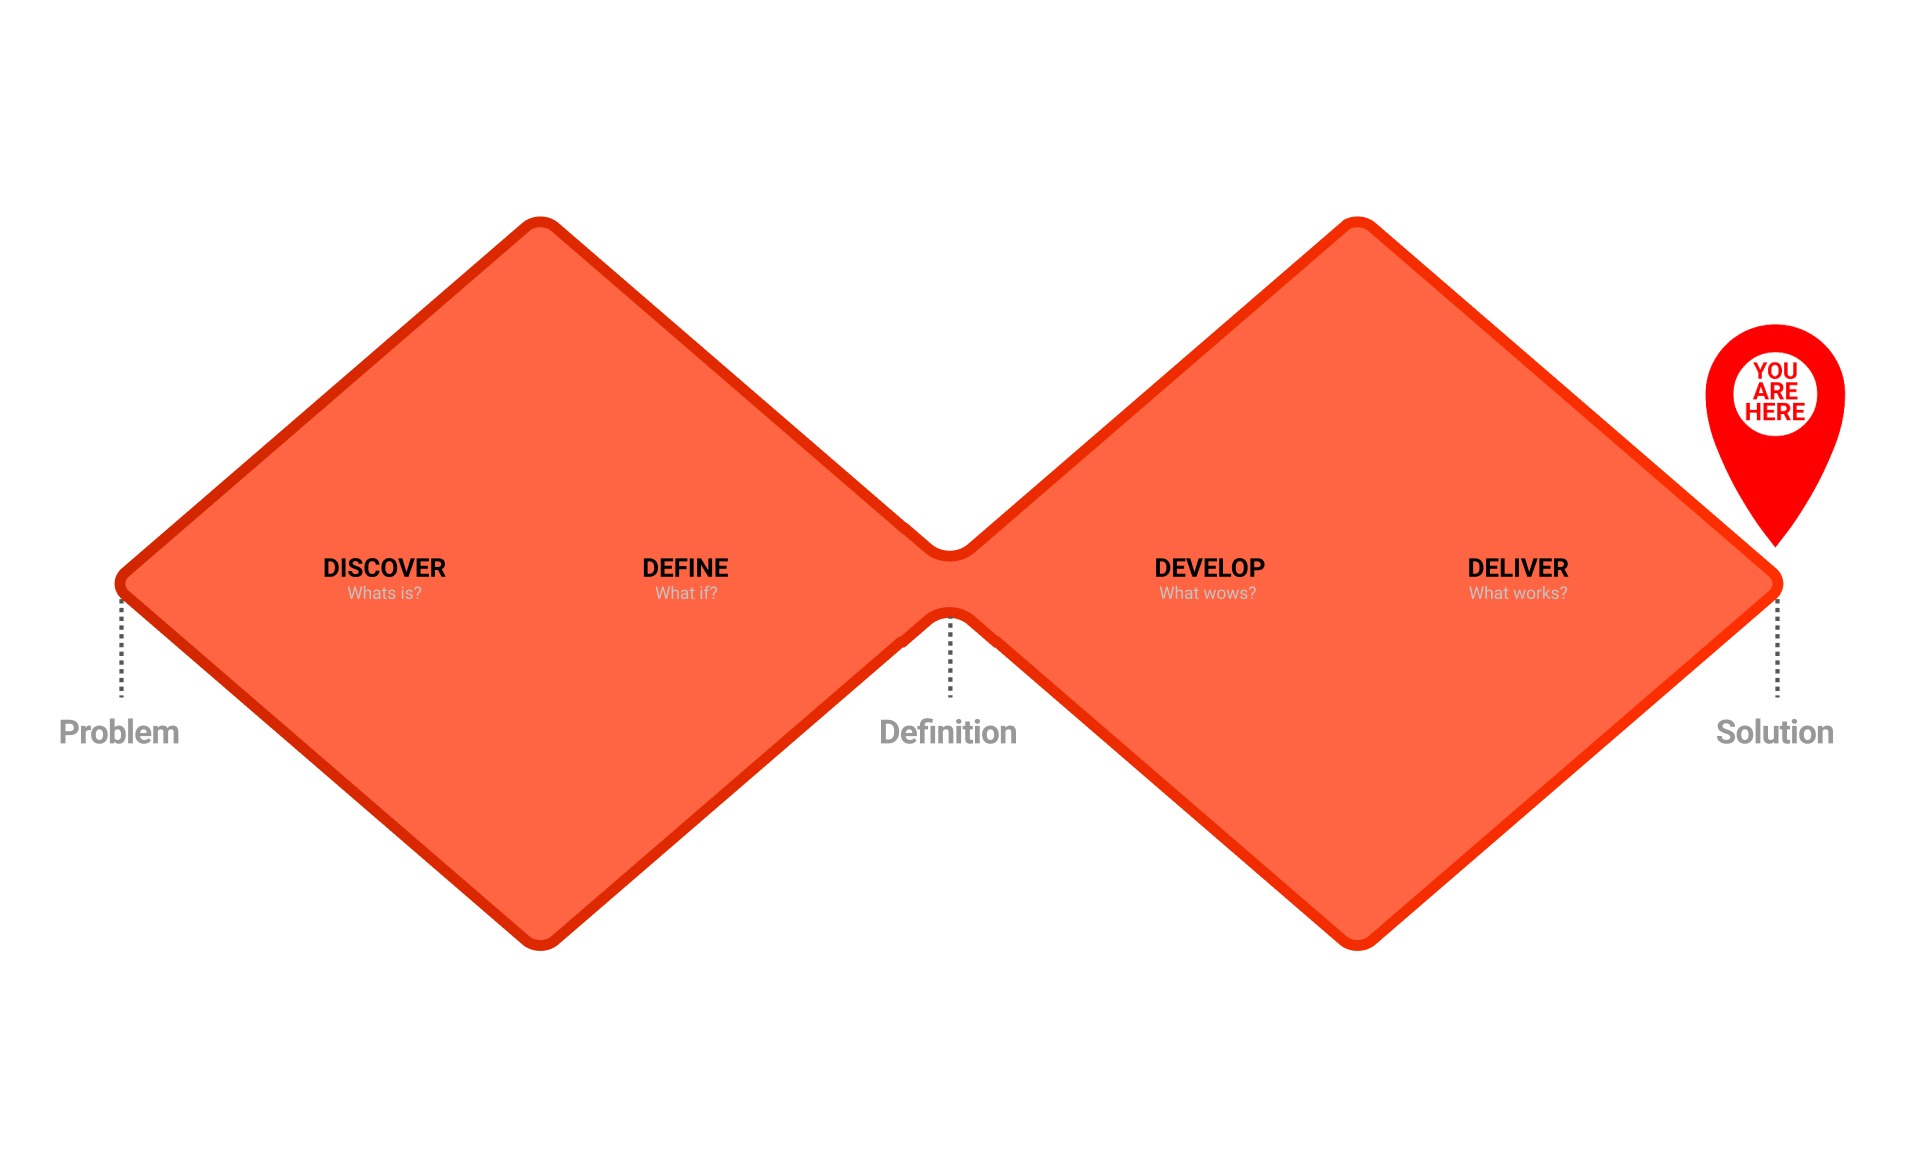
\includegraphics[width=0.9\linewidth]{Imagens/V1 D.jpg}
\end{figure}
\end{frame}


%%%%%%%%%%%%%%%%%%%%%%%%
\section{Code details}
\begin{frame}
\centering \Huge {\currentname}
\end{frame}


\subsection{IoT modules}

\begin{frame}[fragile]
\frametitle{\secname\ - \subsecname\ - ML edge inference}
    \begin{lstlisting}[language=Python]
class Inferencer():
    def __init__(self, path:str, score_threshold:float=0.8):
        self.score_threshold = score_threshold
        path_model = path + 'model.onnx'
        path_labels = path + 'labels.json'
        path_colors = path + 'colors.json'
        self.sess = rt.InferenceSession(path_model)
        ...
    def predict(self, image_bytes:bytes) -> Tuple[List[dict], bytes]:
        ...
        boxes, labels, scores = self.sess.run(
            output_names=output_names,
            input_feed={sess_input[0].name: img_data}
        )
        ...\end{lstlisting}
    "onnxruntime:v.1.4.0-jetpack4.4-l4t-base-r32.4.3" was used as base docker image
\end{frame}

\begin{frame}
\frametitle{\secname\ - \subsecname\ - ML edge inference}
\begin{figure}
    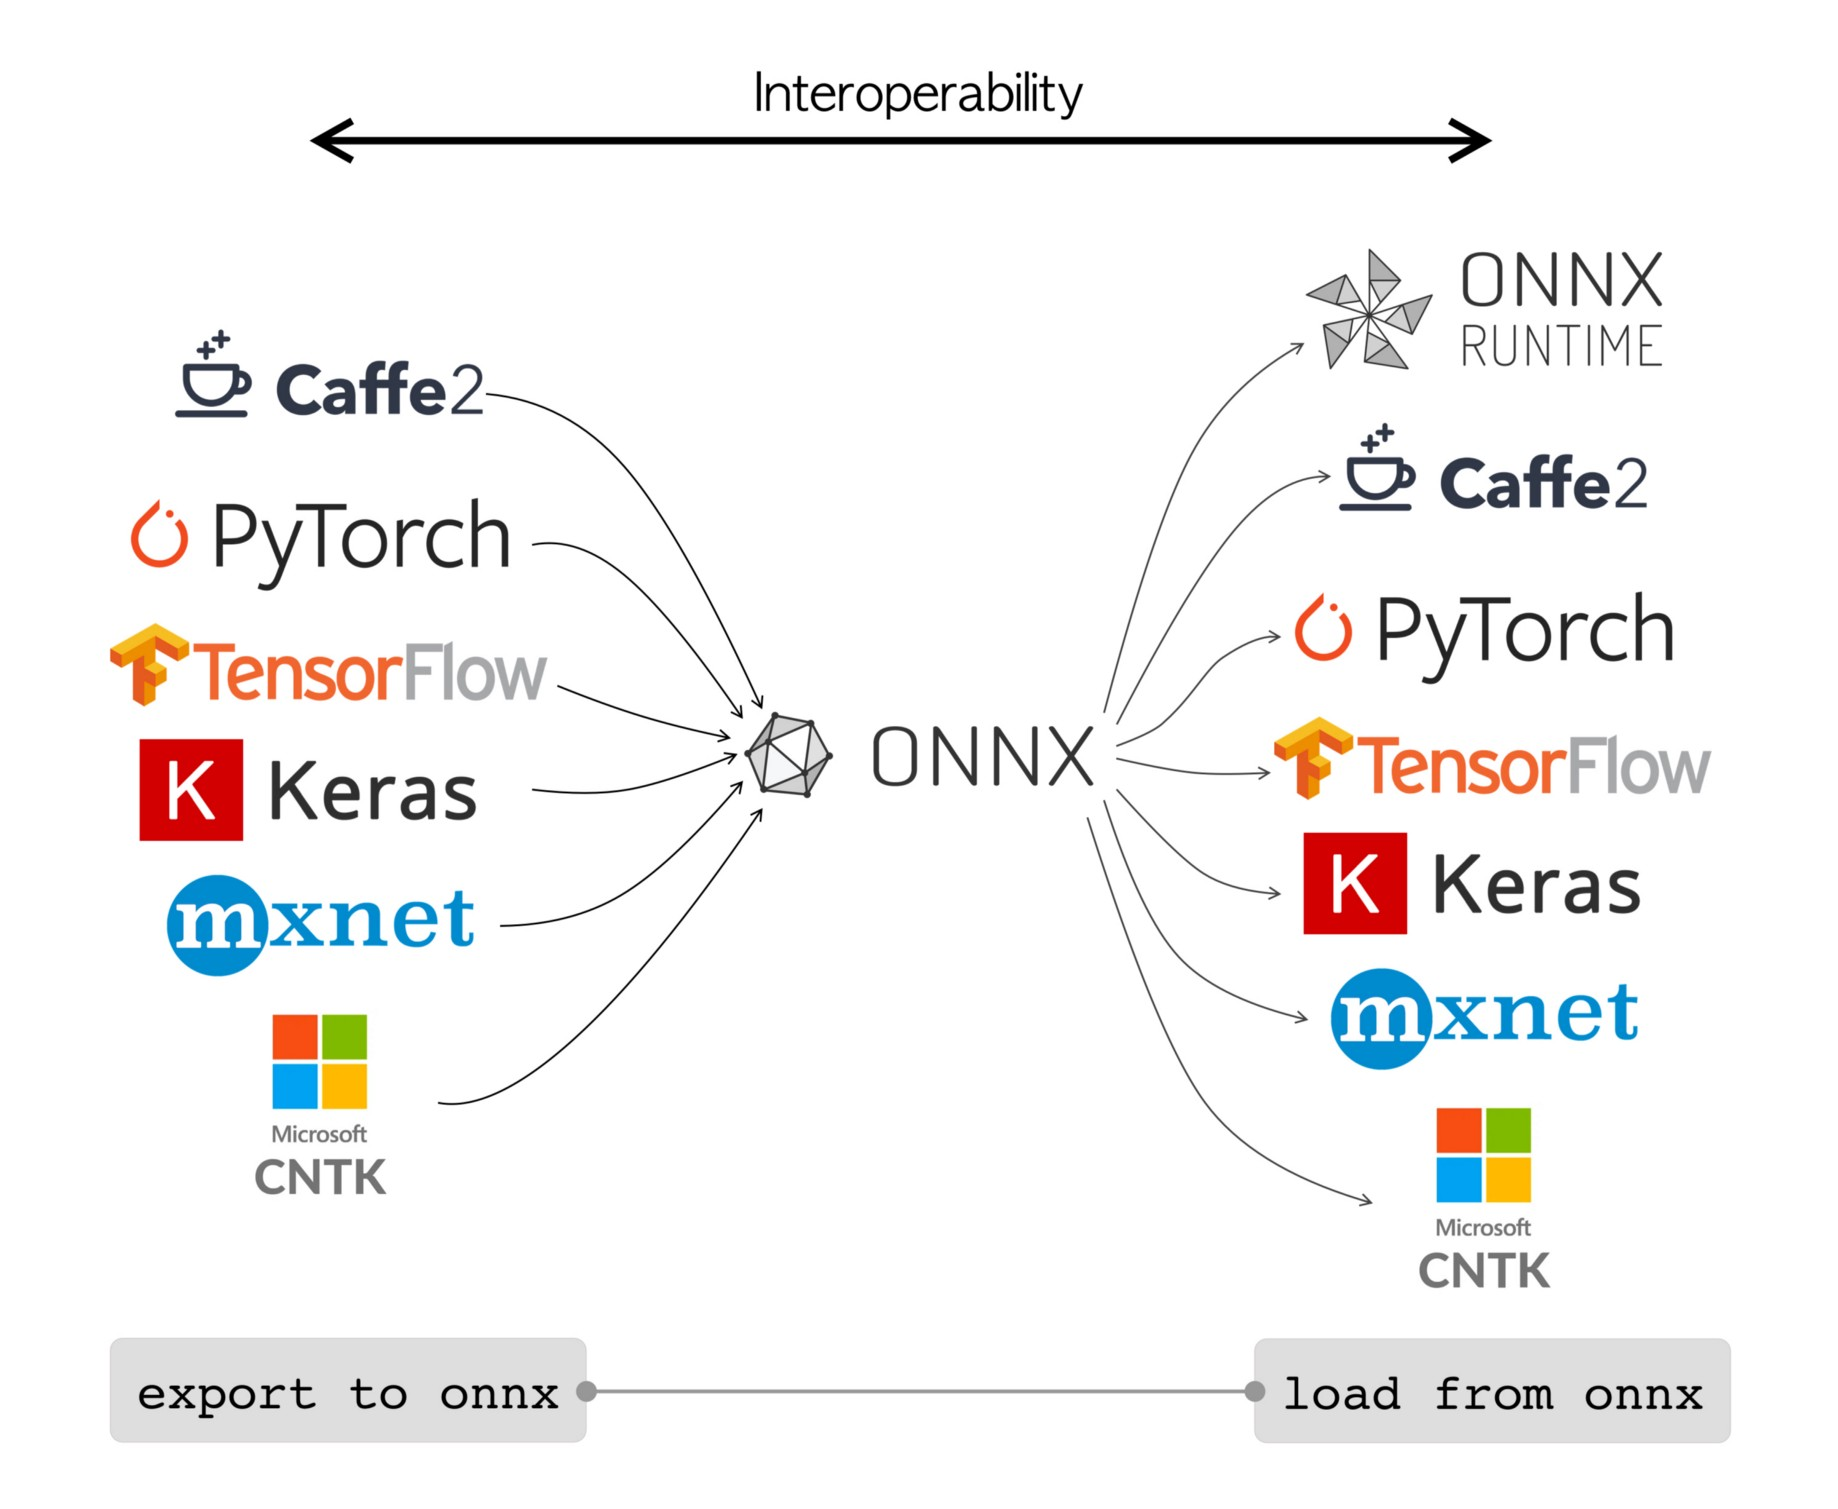
\includegraphics[width=0.7\linewidth]{Imagens/onnx.png}
\end{figure}
\end{frame}

\begin{frame}[fragile]
\frametitle{\secname\ - \subsecname\ - Web server}
    \begin{lstlisting}[language=Python]
@app.post("/inference")
async def inference(image_file: UploadFile = File(...)):
    image_bytes = await image_file.read()
        detections, img_out = app.state.inferencer.predict(image_bytes)

    return StreamingResponse(io.BytesIO(img_out), media_type='image/jpg', headers={'detections': json.dumps(detections)})
    \end{lstlisting}
\end{frame}

\begin{frame}[fragile]
\frametitle{\secname\ - \subsecname\ - ML cloud inference}
    % javascript
    \begin{lstlisting}[language=Java]
// The function is triggered by a file upload (an Azure Event Grid event)
module.exports = async function (context, eventGridEvent) {
...

// Read the uploaded iamge
const img = await loadImage(imageUrl.url);
...

// Predicts calling azure's HTTP API
const predictor = new PredictionApi.PredictionAPIClient(
    predictor_credentials,
    endPoint
);
const results = await predictor.detectImageUrl(
    projectId,
    publishIterationName,
    imageUrl
);
    \end{lstlisting}
\end{frame}

\begin{frame}[fragile]
\frametitle{\secname\ - \subsecname\ - Edge model management}
    \begin{lstlisting}[language=Python]
blob_download_folder(
    connection_string=os.getenv('CLOUD_STORAGE_MODEL_CONNECTION'),
    container='models',
    path_cloud=f'{version}/',  
    path_local='models',
)
    \end{lstlisting}
    
    \begin{lstlisting}[language=HTML]
"Binds": [
    "/home/nano/models:/app/models"
]
    \end{lstlisting}
\end{frame}

%%%%%%%%%%%%%%%%%%%%%%%
\subsection{Infrastructure}

% a dataset of 320 images, the model needs around 38 minutes to train
\begin{frame}[fragile]
\frametitle{\secname\ - \subsecname\ - Azure ML}
\begin{lstlisting}[language=HTML]
resource "azurerm_machine_learning_workspace" "aml" {
  name                    = "aml-workspace"
  location                = azurerm_resource_group.rg.location
  resource_group_name     = azurerm_resource_group.rg.name
  application_insights_id = azurerm_application_insights.appinsights.id
  key_vault_id            = azurerm_key_vault.keyv.id
  storage_account_id      = azurerm_storage_account.storacc.id

  identity {
    type = "SystemAssigned"
  }
}
\end{lstlisting}
\end{frame}

\begin{frame}
\frametitle{\secname\ - \subsecname\ - Azure ML}
\begin{figure}
    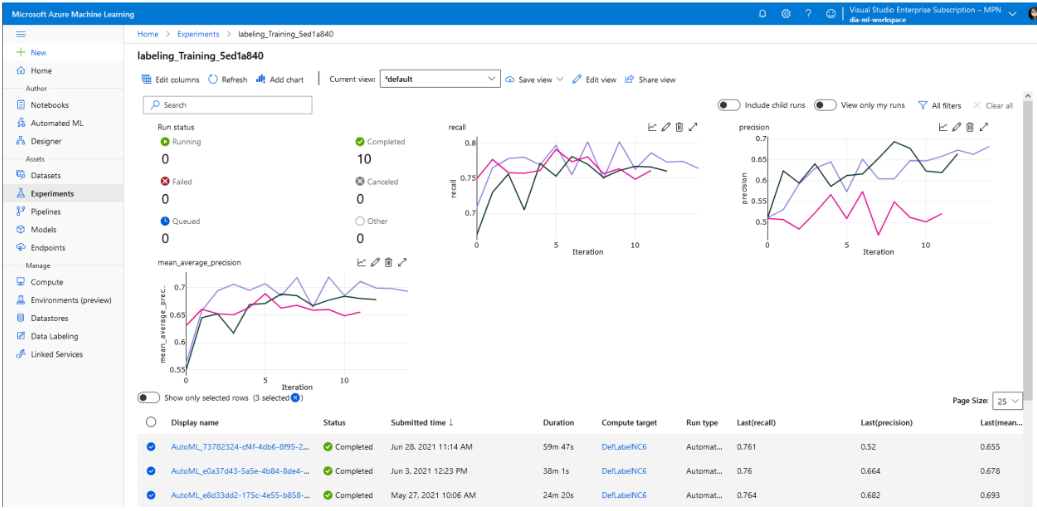
\includegraphics[width=0.9\linewidth]{Imagens/auto_ml.png}
\end{figure}
\end{frame}


\begin{frame}[fragile]
\frametitle{\secname\ - \subsecname\ - DPS}
    \begin{lstlisting}[language=HTML]
resource "azurerm_iothub_dps" "main" {
    name                = var.name_simple
    resource_group_name = azurerm_resource_group.main.name
    location            = azurerm_resource_group.main.location

    sku {
        name     = "S1"
        capacity = 1
    }

    linked_hub {
        connection_string = azurerm_iothub_shared_access_policy.main.primary_connection_string
        location = azurerm_iothub.main.location
    }
}
    \end{lstlisting}
\end{frame}

\begin{frame}
% The device has to prove its identity, but afterwards the uniqye device’s ID is returned by DPS
% $0.10 per 1,000 operations 
\frametitle{\secname\ - \subsecname\ - DPS}
\begin{figure}
    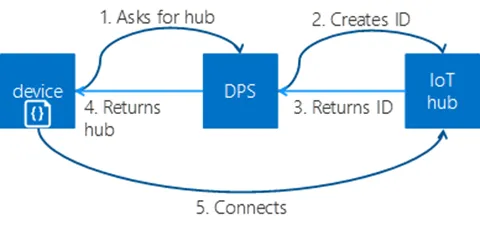
\includegraphics[width=0.5\linewidth]{Imagens/dps.png}
\end{figure}
Source: Martin Abbott, 2017, infoQ.
\end{frame}

%%%%%%%%%%%%%%%%%%%%%%%%
\subsection{CI/CD pipeline}

\begin{frame}[fragile]
\frametitle{\secname\ - \subsecname\ - Apply terraform}
\begin{lstlisting}[language=HTML]
  - task: TerraformTaskV2@2
    displayName: "Terraform apply main ${{ parameters.TF_VAR_ENVIRONMENT }}"
    inputs:
      command: apply
      commandOptions: "-lock-timeout=10m ${{ parameters.TF_VAR_ENVIRONMENT }}-main.plan"
      environmentServiceNameAzureRM: ${{ parameters.azureServiceConnection }}
      workingDirectory: ${{ parameters.workingDirectory }}/base_infra/tf-main/
\end{lstlisting}
\end{frame}

\begin{frame}[fragile]
\frametitle{\secname\ - \subsecname\ - Build containers}
\begin{lstlisting}[language=HTML]
...
\end{lstlisting}
\end{frame}


\begin{frame}[fragile]
\frametitle{\secname\ - \subsecname\ - Deploy modules}
\begin{lstlisting}[language=HTML]
...
\end{lstlisting}
\end{frame}



%%%%%%%%%%%%%%%%%%%%%%%%
\section{References}
\begin{frame}
\frametitle{\currentname}
\begin{itemize}
    \item "Internet of Things From Hype to Reality" Ammar Rayes, Samer Salam
    \item "Agricultural robot dataset for plant classification, localization and mapping on sugar beet fields". Nived Chebrolu and Philipp Lottes and Alexander Schaefer and Wera Winterhalter and Wolfram Burgard and Cyrill Stachniss.
    \item Bosh smart spraying. https://www.bosch.com/research/know-how/success-stories/smart-spraying-precision-herbicide-application-on-weeds/
\end{itemize}
\end{frame}


\end{document}